\documentclass[11pt]{amsart}

\usepackage{amsmath}
\usepackage{physics}
\usepackage{graphicx}
\usepackage{verbatim}

\renewcommand{\thesubsection}{\thesection.\alph{subsection}}

\title[Vibrations and Phonons]{Vibrations and Phonons \\
		\hrulefill \small{ FYS3410: Problem Sheet 2 } \hrulefill}
	
\author{Candidate 33}


\begin{document}

\maketitle

\begin{comment}

\section{Vibrations of a One-Dimensional Monatomic Chain}
This is a study of the vibrations in an infinite one-dimensional crystal with just one atom in  the basis. 

\subsection{Dispersion Relation}
If the temperature of the  crystal is low enough one can model the crystal as a chain of masses held together by springs with length $a$, which is also the lattice constant. Hooke's law can be used to model the force between the atoms,
\begin{equation}
F = g\delta x,
\end{equation}
where $g$ is the spring constant and $\delta x$ is the displacement of a particular mass. Such a model is often referred to as a \emph{harmonic} chain.

The position of atom $n$ in the lattice is $x_n$. The equilibrium position of this atom is $x_n^{eq} = na$. Once we allow for motion of the atoms $x_n$ will deviate from the equilibrium position,
\begin{equation}
\delta x_n = x_n - x_n^{eq}.
\end{equation}
The force acting on mass $n$ in the chain is then given by
\begin{equation}
F_n = g(\delta x_{n+1} - \delta x_n) + g(\delta x_{n-1} - \delta x_n),
\end{equation}
when taking into consideration the atoms of each side of atom $n$. Thus we have Newton's equation of motion
\begin{equation}
\label{eq:N2L}
m(\delta \ddot{x}_n) = F_n = g(\delta x_{n+1} + g(\delta x_{n-1} - 2\delta x_n).
\end{equation}
A good guess to a solution to this equation is
\begin{equation}
\label{eq:oscillatorsolution}
\delta x_n = Ae^{i\omega t - ikx_n^{eq}}=Ae^{i\omega t - ikna},
\end{equation}
where $A$ is the amplitude of the oscillation, and $k$ and $\omega$ are the wavevector and frequency of the proposed wave. The only thing a bit strange here is that there are, apparently, complex values of $\delta x_n$. The complex numbers are used for convenience, but actually the real part of the expression is implied.

Inserting equation \ref{eq:oscillatorsolution} into equation \ref{eq:N2L} yields
\begin{align*}
-m\omega^2Ae^{ik\omega t - ikna} &= gAe^{i\omega t}(e^{-ikna(n+1)} + e^{-ika(n-1)} - 2e^{-ikan}), \\
m\omega^2 &= 2g(1-\cos ka) = 4g\sin^2 \frac{ka}{2}.
\end{align*}
From this the desired result is obtained
\begin{equation}
\omega = 2\sqrt{\frac{g}{m}}\abs{\sin{\frac{ka}{2}}},
\end{equation}
which is a general relationship between a frequency (energy) and a wavevector (momentum) known as a \emph{dispersion relation}.

\subsection{Visualisation of the Dispersion Relation}
One can see from the plot in figure \ref{fig:brillouin_dispersion} how the dispersion relation repeats after the first Brillouin zone, indicated by dashed lines. The dispersion is in fact periodic in $k \rightarrow k + 2\pi/a$. When one knows the dispersion relation for the first Brillouin zone, one knows the dispersion relation everywhere.

\begin{figure}
\centering
	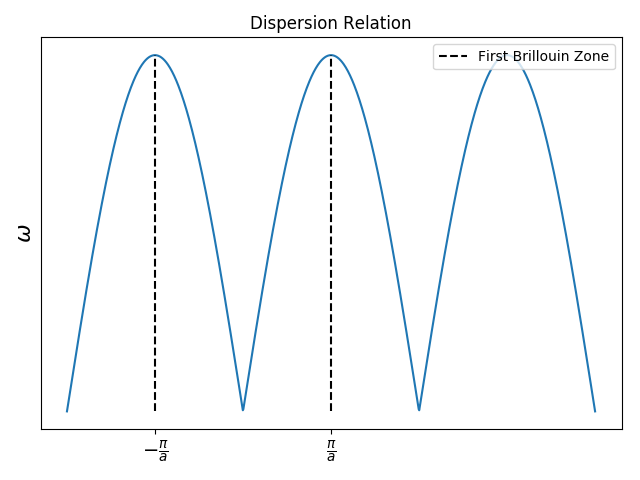
\includegraphics[width=0.7\textwidth]{first_brillouin.png}
	\caption{The dispersion relation is repeated after the first Brillouin zone.}
	\label{fig:brillouin_dispersion}
\end{figure}

\subsection{Group Velocity}
The group velocity is given by
\begin{equation}
v_g = \frac{\Delta \omega}{\Delta k},
\end{equation}
for an infinitesimal change this is equal to the derivative of the dispersion relation with regards to $k$. By looking at the graph in figure \ref{fig:brillouin_dispersion}, one can see that the group velocity must be highest at the center of the first Brillouin zone. The group velocity is decreasing towards zero as one gets closer to the edge of the first Brillouin zone. 

\subsection{Maximum Amplitude of Na-crystal}
Imagine a longitudinal wave propagating in direction [100], given by Miller indices, in a sodium (Na) crystal.

Limiting the viewpoint again to the  first Brillouin zone ($k\pm+pi/a$) gives a standing wave defined by 
\begin{equation}
\delta_n = Ae^{i\omega t - ikna}
\end{equation}

\end{comment}

\setcounter{section}{1}
\section{Density of States (DOS) for Phonons}
The phonon density of states in a one-dimensional array of $N$ atoms is derived in the following.

\subsection{DOS as a function of wave-vector}
One can view the one-dimensional array of atoms as a ring where the first and the last atom is connected to each other. Such a boundary condition is known as a Born-von Karman boundary condition. This boundary implies that atom number $n$ is the same atom as atom number $n+N$.
The displacement of this atom is
\begin{equation*}
\delta x_n = \delta x_{n+N}.
\end{equation*}
Applying Bloch's theorem\footnote{$\psi(\vb{r}+\vb{R})=e^{i\vb{k}\cdot\vb{R}}\psi(\vb{r})$}
to this relation gives
\begin{equation*}
\delta x_1 e^{ikan} = \delta x_1 e^{ika(n+N)},
\end{equation*}
where $k$ is the wave-vector and $a$ is the lattice parameter. To satisfy this condition we must have
\begin{equation*}
1 = e^{ikaN} = \cos(kaN) + i\sin(kaN),
\end{equation*}
which only is satisfied if
\begin{equation*}
2\pi\nu = kaN, \quad \nu=1,2,\dots,N
\end{equation*}
which gives
\begin{equation*}
k = \frac{2\pi}{Na}\nu.
\end{equation*}
The separation between allowed solution ($k$-values) is therefore
\begin{equation}
\Delta k = \frac{2\pi}{Na}.
\end{equation}
Thus, in one dimension the density of states is
\begin{equation}
D(k) = \frac{1}{\Delta k} = \frac{Na}{2\pi} = \frac{L}{2\pi}.
\end{equation}
One can easily see that the density of states (DOS) is independent of $k$, so the density of modes in $k$-space is uniformly distributed.

\subsection{DOS as a function of angular frequency}
A one-dimensional lattice with one atom in the basis can be modelled as a harmonic chain, where one imagines a spring connecting all the atoms. The dipsersion relation then becomes
\begin{equation}
\label{eq:disprel}
\omega = \omega_0\sin{\frac{ka}{2}}, \quad \omega_0 = 2\sqrt{\frac{g}{m}}
\end{equation}
where $\omega$ is the angular frequency, $g$ is the spring constant and $m$ is the mass of each atom.

One can change between one density of states to the other by way of the following formula
\begin{equation}
D(\omega)d\omega = D(k)dk = \frac{Na}{2\pi}dk.
\end{equation}
which can be rewritten to include the group velocity
\begin{equation}
\label{eq:insertgrouphere}
D(\omega)d\omega = \frac{Na}{2\pi}\frac{dk}{d\omega}d\omega = \frac{Na}{2\pi}\frac{d\omega}{v_g}.
\end{equation}
The group velocity is
\begin{equation}
\label{eq:groupvel2}
v_g = \frac{dw}{dk} = \omega_0\frac{a}{2} \cos{\frac{ka}{2}}.
\end{equation}
This equation is to be inserted in equation \ref{eq:insertgrouphere}, but first we also need a function of $\omega$ instead of $k$ which is found by inverting equation \ref{eq:disprel}
\begin{align*}
\omega &= \omega_0\sin{\frac{ka}{2}} \\
\frac{\omega}{\omega_0} &= \sin{\frac{ka}{2}} \\
\frac{ka}{2} &= \arcsin{\frac{\omega}{\omega_0}} \\
k &= \frac{2}{a}\arcsin{\frac{\omega}{\omega_0}}.
\end{align*}
This can now be inserted into the group velocity
\begin{align*}
v_g &= \omega_0\frac{a}{2}\cos\left(\frac{a}{2}\frac{2}{a}\arcsin\frac{\omega}{\omega_0} \right) \\
	&= \omega_0\frac{a}{2}\sqrt{1-\left(\frac{\omega}{\omega_0}\right)^2}.
\end{align*}
inserting this expression into \ref{eq:insertgrouphere} yields
\begin{equation}
D(\omega) = \frac{N}{\pi\omega_0}\frac{1}{\sqrt{1-\left(\frac{\omega}{\omega_0}\right)^2}}
\end{equation}
which is the density of states as a function of angular frequency.

\subsection{Comparison of DOS measures}
\begin{figure}
\centering
	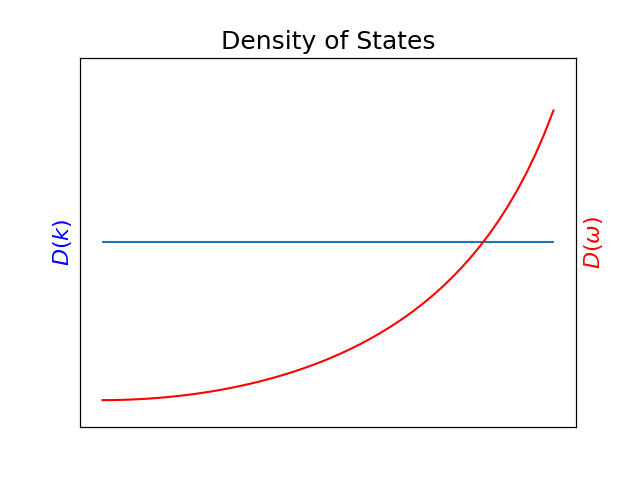
\includegraphics[width = 0.9\textwidth]{DOS.png}
	\caption{Comparison of density of states. $D(k)$ on the left axis and $D(\omega)$ on the right.}
	\label{fig:DOS}
\end{figure}

A comparison of the two DOS measures that has been derived is shown in figure \ref{fig:DOS}. The first $y$-axis is used for $D(k)$, and the second for $D(\omega)$. Because the density of states for $k$, $D(\omega)$ is constant for all $k$, this is much easier to deal with than the ever changing $D(\omega)$. The much more stable density of states i $k$-space is reason enough to use $D(\omega)$, but this one also has a closer connection with reciprocal space and diffraction patterns.

\section{Different Models for Temperatur-Heat Capacity Dependence}
In the outline of the following models I will be very brief, and not fully derive the models, but rather give a more qualitative description.

\subsection{Dulong-Petit}
The Dulong-Petit law is a thermodynamic rule proposed in 1819 by French physicists Pierre Louis Dulong and Alexis Thérèse Petit. They assume that every mode oscillates according to a classical harmonic oscillator, with continuous energy. In such a classical treatment, the thermal energy density is
\begin{equation}
u = \frac{1}{V}\frac{\int dV e^{-\beta H}H}{\int dV e^{-\beta H}} = -\frac{1}{V}\frac{\partial}{\partial \beta}\ln \int dV e^{-\beta H}
\end{equation}
where $\beta = 1/k_BT$ and $H$ is the enthalpy. By making a change of variables, one finds that the integral equates to
\begin{equation}
u = u_{eq} + 3nk_BT,
\end{equation}
which yields the heat capacity
\begin{equation}
C_v = \frac{\partial u}{\partial T} = 3nk_B.
\end{equation}
The heat capacity is a straight line, and measured heat capacities come quite close to the Dulong and Petit value. However, when temperature drops, the heat capacity falls well below the Dulong and Petit value. Moreover, when the temperature gets large, it seems fairly clear that the curve never quite reaches the precise value, as can be seen in figure 		\ref{fig:dulongpetit}. In conclusion, the law of Dulong and Petit is a reasonable approximating for higher temperatures.

\begin{figure}
\centering
	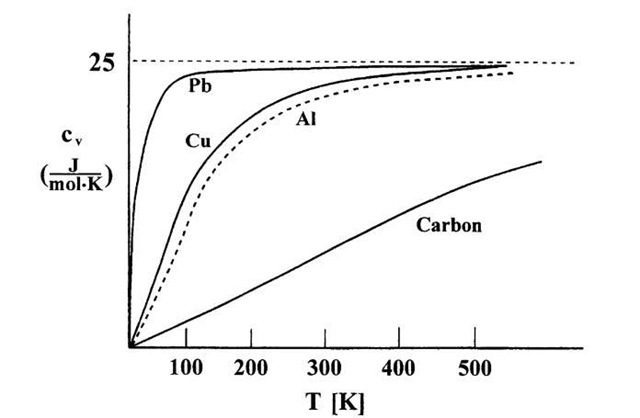
\includegraphics[width = 0.8\textwidth]{dulong_petit.jpg}
	\caption{Measured heat capacities for lead, copper, aluminimum and carbon. The horizontal line is the classical Dulong and Petit value.}
	\label{fig:dulongpetit}
\end{figure}

\subsection{Einstein}
The Einstein model for the solid employs quantum harmonic oscillators (QHO), where the eigenvalue energies of a single oscillator is
\begin{equation}
E_n = \hbar\omega\left(n\frac{1}{2}\right).
\end{equation}
Furthermore, the model assumes that the atoms in the crystal are non-interaction.

The main difference from the Dulong and Petit model, however, is that the QHO energy levels are quantized, as $n$ in the equation above can only have integer values. 

In one dimension the partition function becomes
\begin{equation}
Z_{1D} = \sum e^{-\beta\hbar\omega (n+1/2)},
\end{equation}
and from this stems the expected energy
\begin{equation}
\ev{E} = -\frac{1}{Z_{1D}}\frac{\partial Z_{1D}}{\partial \beta} = \frac{\hbar\omega}{2}\coth\left(\frac{\beta\hbar\omega}{2} \right) = \hbar\omega\left(n_B(\beta\hbar\omega) +\frac{1}{2} \right),
\end{equation}
where $n_B$ is the Bose occupation factor
\begin{equation*}
n_B = \frac{1}{e^x-1}.
\end{equation*}
It is easy to fathom that $\ev{E_{3D}} = 3\ev{E_{1D}}$, as each atom is oscillating in all three dimensional directions. Thus, the heat capacity becomes
\begin{equation}
C_v(T) = \frac{\partial \ev{E_{3D}}}{\partial T} = 3_kB(\beta\hbar\omega)^2\frac{e^{\beta\hbar\omega}}{(e^{\beta\hbar\omega} -1)^2},
\end{equation}
where it is traditional to define the Einstein temperature as $T_{Eintstein}=\hbar\omega / k_B$. We can see that this expression \emph{does} depend on the temperature.

The Einstein model uses quantized energy levels and as a consequence becomes dependent on temperature. The heat capacity derived from this model becomes similar to the Petit and Dulong value for hight temperatures, but will fall as the temperature get lower. This is more in accordance with the experimental data shown in figure \ref{fig:dulongpetit}. However, the heat capacity values provided by the model was found to fall too quickly for the very lowest temperatures.

\subsection{Debye}
Petrus Josephus Wilhelmus Debije\footnote{Yes, that is is original name. He changed the way he wrote it at some point in his life.} theorised that the oscillation modes of a solid were waves with frequencies $\omega(\vb{k}) = v\abs{\vb{k}}$ with $v$ the sound velocity. For each $\vb{k}$ there are three possible oscillation modes, one for each dimension. This enables one to write an expression entirely analogous to Einstein's expression
\begin{equation}
\label{eq:debyestart}
\ev{E} = 3\sum_k\hbar\omega(\vb{k})\left(n_b(\beta\omega(\vb{k}))+\frac{1}{2}\right).
\end{equation}
This sum can be approximated by an integral\footnote{The full derivation of this model is given in the final section of this document.} eventually finding
\begin{equation}
C_v = \frac{\partial\ev{E}}{\partial T} = Nk_B \frac{(k_B T)^3}{(\hbar\omega_d)^3}\frac{12\pi^4}{4} \propto T^3.
\end{equation}
The Debye frequency, $\omega_d$ in this expression is sometimes replaced by the Debye temperature, $T_{Debye} = \hbar\omega_d/k_B$.

Because the oscillations of the Debye models give slightly different results than that of the Einstein model, the Debye model yields better results than the Einstein model at low temperatures. See figure \ref{fig:debyeVSEinstein} for a comparison.

\begin{figure}
\centering
	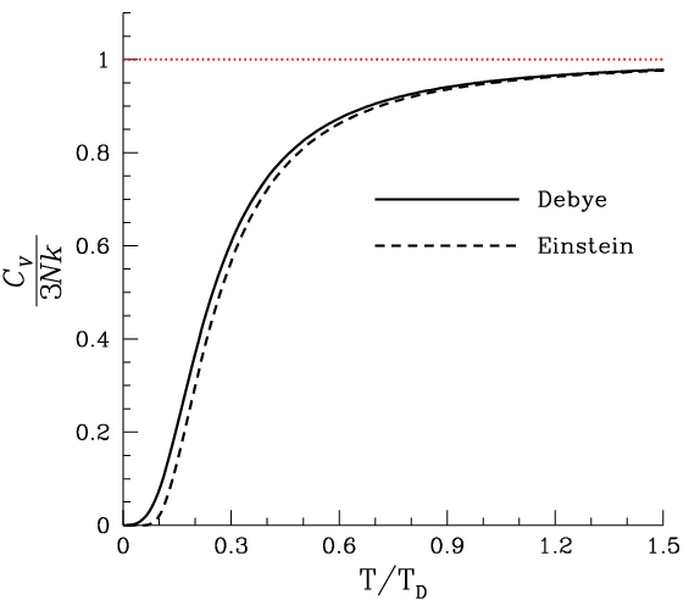
\includegraphics[width = 0.7\textwidth]{DebyeVSEinstein.jpg}
	\caption{A comparison of the Einstein and Debye models for heat capacity.}
	\label{fig:debyeVSEinstein}
\end{figure}

\setcounter{section}{5}
\section{Thermal Conductivity}

\end{document}